中国的甭管是《高等代数》还是《线性代数》一般都是从行列式开始讲的,但是老外的课本一般都是
从矩阵或者方程组开始讲的。所以很多人说我们中国人课本不讲道理,莫名其妙就来了个行列式,首
先第一个问题:为什么要引入行列式这么一个概念?这就得从方程组开始说起。假设我们解一个二元
一次方程组
$$\begin{cases}
    3x+4y=5 & \text{\ding{172}}\\
    7x+9y=11 & \text{\ding{173}}
\end{cases}$$
这是一个二元一次线性方程组,大家会的就是消元法,所以我们就开始消元。首先消去$y$,将\ding
{172}$\times 9$;\ding{173}$\times 4$,于是得到了
$$\begin{cases}
    3\times 9x+4\times 9y=5\times 9 & \text{\ding{174}}\\
    7\times 4x+9\times 4y=11\times 4 & \text{\ding{175}}
\end{cases}$$
然后我们用\ding{174}$-$\ding{175},就能将$y$消去,得到了
\[(3\times 9-7\times 4)x=5\times 9-11\times 4\]
所以,经过移项可得
\[x=\dfrac{5\times 9-11\times 4}{3\times 9-7\times 4}\]
这样就得到了$x$。同样的,也可以采用类似的方法消去$x$而得到$y$,这里我(宋老师)就不写一遍
了。如果将$x$消去,那么就可以得出
\[y=\dfrac{3\times 11-5\times 7}{3\times 9-7\times 4}\]

如果我们就这样把结果计算出来是可以的,但是我们看下最终结果的这个形式它是有规律的。甭管它的
分子还是分母都是两个数相乘减两个数相乘的形式。这时候我们就把这种形式给它定义成一个新的符号
,形式如下:
\begin{align*}
    x=\dfrac{\begin{vmatrix} 5 & 11\\ 4 & 9\end{vmatrix}}
            {\begin{vmatrix} 3 & 7\\ 4 & 9\end{vmatrix}} \qquad\qquad
    y=\dfrac{\begin{vmatrix} 3 & 5\\ 7 & 11\end{vmatrix}}
            {\begin{vmatrix} 3 & 7\\ 4 & 9\end{vmatrix}}
\end{align*}

这就相当于我们定义了一个新的运算,与我们初中、高中的“新定义”题型类似。也就是说可以写出如下
这种两行两列,两边加上两根竖线的形式。并且定义其运算规则为:
\begin{align*}
    \begin{vmatrix}
        a & b \\
        c & d
    \end{vmatrix}=ad-bc.
\end{align*}
这样我们就引入了一个新的运算,就将原来的分子分母变成了新的形式。我们引入这种新的运算的目的就
是为了更方面的表达形如$5\times 9-11\times 4$这种形式的数。

\begin{wrapfigure}{r}{.3\textwidth}
    \centering
    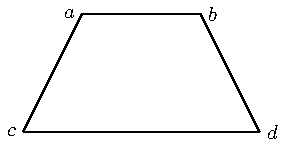
\includegraphics{images/1.1.pdf}
    \caption{}
    \label{pic:1.1}
\end{wrapfigure}

那为什么要搞成两根竖线的形式呢?为什么不能是如\figref{pic:1.1}这样的形式呢?(\textcolor
{cyan}{\heiti 抱歉,各位,宋老师那个很骚的带花边的我实在无能为力}.)行啊,当然可以,只不过
最早发明这个定义的人采用了前面所示的方法来表示的,并且这个符号也比较简洁。所以,就引出了这样
一个行列式,所以行列式就是这么来的。

接下来,我们就可以给出二阶行列式的定义了。

\begin{definition}[二阶行列式]\label{def:1.1}
    我们将形如
    \begin{align}
        \begin{vmatrix}
            a_{11} & a_{12}\\
            a_{21} & a_{22}
        \end{vmatrix}
    \end{align}
    的式子叫做{\heiti 二阶行列式},它表示2行2列4个元素具有
    \[a_{11}a_{22}-a_{12}a_{21}\]
    这样的关系。
\end{definition}

通过二阶行列式的定义的可以看出,它的最终结果是一个数。所以,你记着,甭管它是二阶行列式还是三阶
行列式、四阶行列式,任何一个行列式的最终结果是一个数。它的样子看起来挺吓人,但经过计算的最终结
果一定是一个数。

定义中的$a_{ij}$的写法中的$i$表示它的行标、$j$表示它的列标。比如:$a_{22}$表示它是第 2 行
第 2 列的元素。这里下标不能读作“二十二”,应该读作“一一、一二、二一、二二”。如果是一个$n$阶的
,比如$a_{39}$表示第 3 行,第 9 列的元素,这就是行标和列标的概念。

$$\left|\:\begin{NiceMatrix}
    1 & 2\\
    3 & 4
    \CodeAfter
        \tikz \draw[red!80,line width=1pt,-latex] (1-1) -- (2-2);
        \tikz \draw[cyan!80,line width=1pt,-latex] (2-1) -- (1-2);
\end{NiceMatrix}\:\right|$$

行列式中从左上角到右下角[如红色箭头所示]叫做{\heiti 主对角线},从左下角到右上角[如蓝色箭头所
示]叫做{\heiti 副对角线}(也叫次对角线)。二阶行列式比较简单,就是主对角线的两个元素相乘减去副
对角线的两个元素相乘。

\vfill
\begin{example}\label{exp:1.1}
    计算$\begin{vmatrix}
        1 & -3\\
        2 & 5
    \end{vmatrix}$
\end{example}
\begin{solution}
    根据二阶行列式的定义
    \[\begin{vmatrix} 1 & -3\\ 2 & 5\end{vmatrix}=1\times 5-2\times(-3)=5+6=11\]
\end{solution}

通过例\ref{exp:1.1}可以看出,任何一个行列式经过计算,其结果都是一个数。我们一定要明白其本质,
比如矩阵,它就是一个矩阵,但是行列式其实是一个数。

\vfill
\begin{example}\label{exp:1.2}
    已知$\begin{vmatrix}
        \lambda-1 & 2\\
        3 & \lambda+4 
    \end{vmatrix}=0$,求$\lambda$。
\end{example}
\begin{solution}
    由行列式定义可知:
    \[(\lambda -1)(\lambda +4)-2\times 3=0,\]
    化简可得:$\lambda^2+3\lambda-10=0$,解得$\lambda=-5$或$\lambda=2$。
\end{solution}

\vfill
\begin{example}\label{exp:1.3}
    解方程组$\begin{cases}
        2x+3y=1\\
        3x+4y=-2
    \end{cases}$
\end{example}
\begin{solution}
    这里使用初中的消元法可以得出结果,但是我们已经学过行列式了。肯定得换个玩法,这是 2 个 2 元
    线性方程组,它有什么特点呢?它有两未知数$x$和$y$且有两方程,这个是我们以后要讲的(克莱姆法则
    Cramer)。那这个东西怎么做呢?这里其实是一个公式,记住就行。首先将未知数$x,y$的系数写作
    \[D=\begin{vmatrix}
        2 & 3\\
        3 & 4
    \end{vmatrix}=2\times 4-3\times 3=8-9=-1\]
    然后用方程右边的数$(1,-2)$去替换$D$中的第 1 列,并记为
    \[D_1=\begin{vmatrix}
        1 & 3\\
        -2 & 4
    \end{vmatrix}=1\times 4-(-2)\times 3=4+6=10\]
    再然后用方程右边的数$(1,-2)$去替换$D$中的第 2 列,并记为
    \[D_2=\begin{vmatrix}
        2 & 1\\
        3 & -2
    \end{vmatrix}=2\times(-2)-3\times 1=-4-3=-7\]
    接着使用公式:
    \[x=\dfrac{D_1}{D}=-10,\quad\quad y=\dfrac{D_2}{D}=7.\]
\end{solution}

\begin{remark}
    $D$是未知数的系数组成的行列式所得到的结果,并且永远在分母上.求$x$则将方程右边的数去替换$x$
    的系数(第一列)所得行列式$D_1$写在分子上,然后得出$x$的值;$y$同理,用方程右边的数去替换$y$
    的系数(第二列)所得行列式$D_2$写在分子上,然后得出$y$的值.
\end{remark}

本节介绍了二阶行列式从何而来,以及二阶行列式的定义。既然有二阶,就会有三阶,那么下一节就将介绍三
阶行列式。